
\section{Experimental Study} 
\label{sec:exp}

Detail the experimental setup used to test the different algorithms. Present the results in an understandable manner (graphics, tables, etc.). Draw conclusions about what things worked (and why) and which didn't (and why). 

\subsection{Evolutionary Algorithm} 


\begin{table}[H]
\caption{}
\begin{tabular}{*9c}  \hline
\multicolumn{1}{p{1cm}}{\centering ID} & 
\multicolumn{1}{p{2cm}}{\centering Safety\\ Iterations} & 
\multicolumn{1}{p{1cm}}{\centering Path Length} & 
\multicolumn{1}{p{1cm}}{\centering Size of\\ Pop.} & 
\multicolumn{1}{p{1cm}}{\centering Fittest\\ Pop.} & 
\multicolumn{1}{p{1cm}}{\centering Dyn. Path\\ Length} & 
\multicolumn{1}{p{1cm}}{\centering Min. Gen.} & 
\multicolumn{1}{p{1cm}}{\centering Avg\\ Wins	} & 
\multicolumn{1}{p{1cm}}{\centering Std of Wins} \\ \hline
1 & 2 & 6 & 14 & 5 & 0 & 4 & 0.459 & 0.023 \\ \hline
2 & 4 & 6 & 10 & 4 & 0 & 4 & 0.458 & 0.024 \\ \hline
3 & 5 & 4 & 14 & 5 & 0 & 4 & 0.466 & 0.028 \\ \hline
4 & 5 & 6 & 10 & 5 & 0 & 4 & 0.459 & 0.032 \\ \hline
5 & 5 & 6 & 13 & 4 & 1 & 5 & 0.451 & 0.041 \\ \hline
6 & 5 & 6 & 14 & 3 & 0 & 4 & 0.471 & 0.018 \\ \hline
7 & 5 & 6 & 14 & 5 & 0 & 4 & 0.461 & 0.025 \\ \hline
8 & 5 & 6 & 14 & 5 & 1 & 2 & 0.479 & 0.021 \\ \hline
9 & 5 & 6 & 14 & 5 & 1 & 4 & 0.463 & 0.027 \\ \hline
10 & 5 & 6 & 14 & 5 & 1 & 6 & 0.449 & 0.041 \\ \hline
11 & 5 & 6 & 14 & 7 & 0 & 4 & 0.474 & 0.028 \\ \hline
12 & 5 & 6 & 18 & 5 & 0 & 4 & 0.462 & 0.035 \\ \hline
13 & 5 & 8 & 14 & 5 & 0 & 4 & 0.453 & 0.029 \\ \hline
14 & 8 & 6 & 14 & 5 & 0 & 4 & 0.477 & 0.022 \\ \hline
\end{tabular}
\label{ea_result}
\end{table}




\begin{figure}
\centering
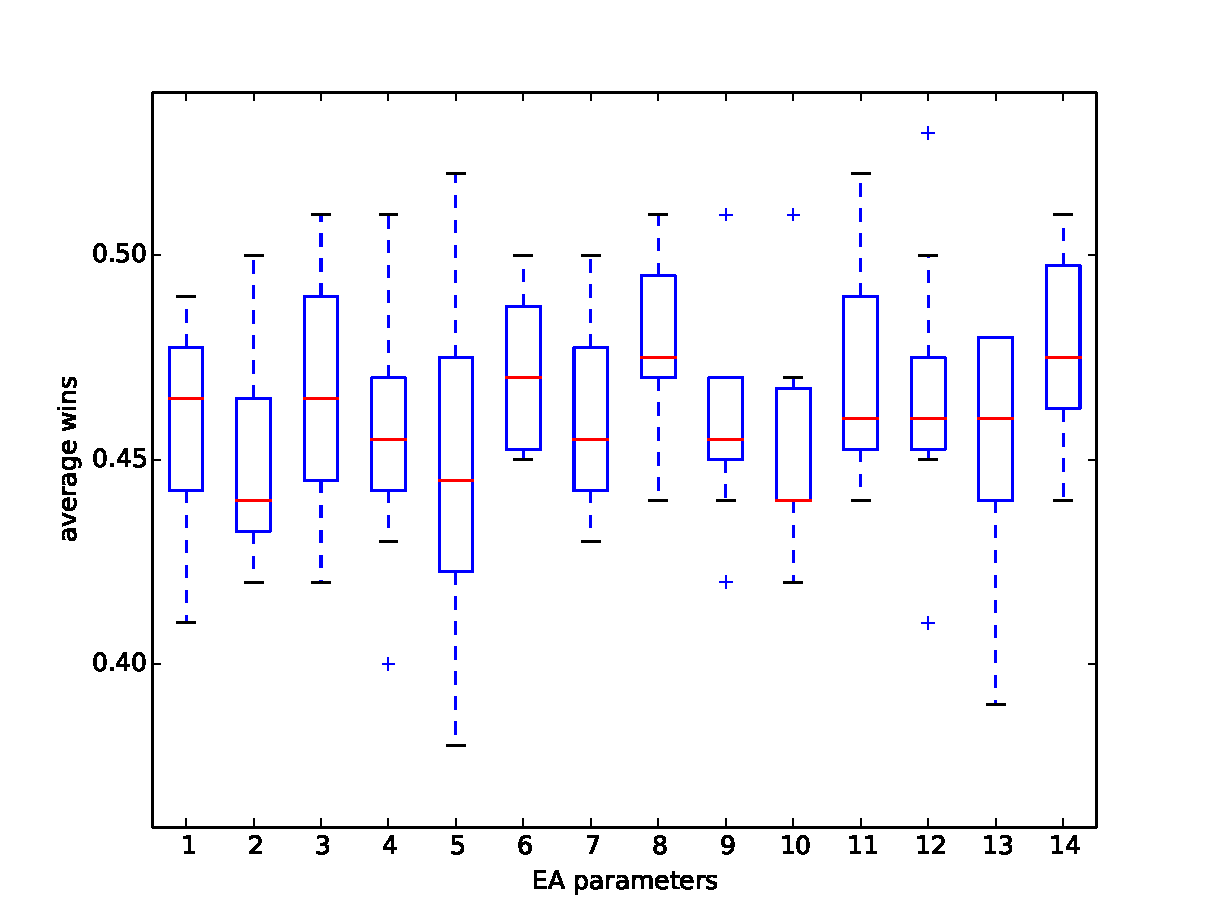
\includegraphics[scale=0.7]{images/eval_evolutionary.pdf}
\caption{result of the evolutionary algorithms}
\label{fig:eval_evo}
\end{figure}





\subsection{General} 